% Created 2016-09-07 Wed 11:46
\documentclass[12pt]{article}
\usepackage[utf8]{inputenc}
\usepackage[T1]{fontenc}
\usepackage{fixltx2e}
\usepackage{graphicx}
\usepackage{longtable}
\usepackage{amsmath}
\usepackage{textcomp}
\usepackage{marvosym}
\usepackage{wasysym}
\usepackage{amssymb}
\usepackage[xetex,bookmarksnumbered,pdfpagelabels=true,colorlinks=true,plainpages=false]{hyperref}
\tolerance=1000
\usepackage{fullpage}
\usepackage{indentfirst}
\usepackage[indentafter,pagestyles]{titlesec}
\usepackage{tabu}
\usepackage{minted}
\usepackage{xltxtra}
\usepackage{xeCJK}
\tolerance=1000
\setlength{\parindent}{2em}
\setmainfont{Liberation Serif}
\setsansfont{Liberation Sans}
\setCJKmainfont[BoldFont={Adobe Heiti Std}]{Adobe Song Std}
\setCJKsansfont{Noto Sans CJK SC Regular}
\setCJKfamilyfont{hei}{Adobe Heiti Std}
\setCJKfamilyfont{song}{Adobe Song Std}
\setCJKfamilyfont{kai}{Adobe Kaiti Std}
\newCJKfontfamily\quotefont{Adobe Kaiti Std}
\XeTeXlinebreaklocale "zh"
\XeTeXlinebreakskip = 0pt plus 1pt
\graphicspath{{./figs/}{../figs/}{./}{../}}
\renewcommand{\contentsname}{目录}
\renewcommand{\listfigurename}{插图目录}
\renewcommand{\listtablename}{表格目录}
\renewcommand{\abstractname}{摘要}
\renewcommand{\appendixname}{附录}
\renewcommand{\indexname}{索引}
\renewcommand{\figurename}{图}
\renewcommand{\tablename}{表}
\author{WANG Xiaolin}
\date{\today}
\title{Play With Bash}
\hypersetup{
  pdfkeywords={bash, shell-scripting, linux},
  pdfsubject={A basic bash tutorial by examples},
  pdfcreator={Emacs 24.5.1 (Org mode 8.2.10)}}
\begin{document}

\maketitle
\tableofcontents


\section{Basic Bash Command Line Operations}
\label{sec-1}
\subsection{Understanding The File System}
\label{sec-1-1}

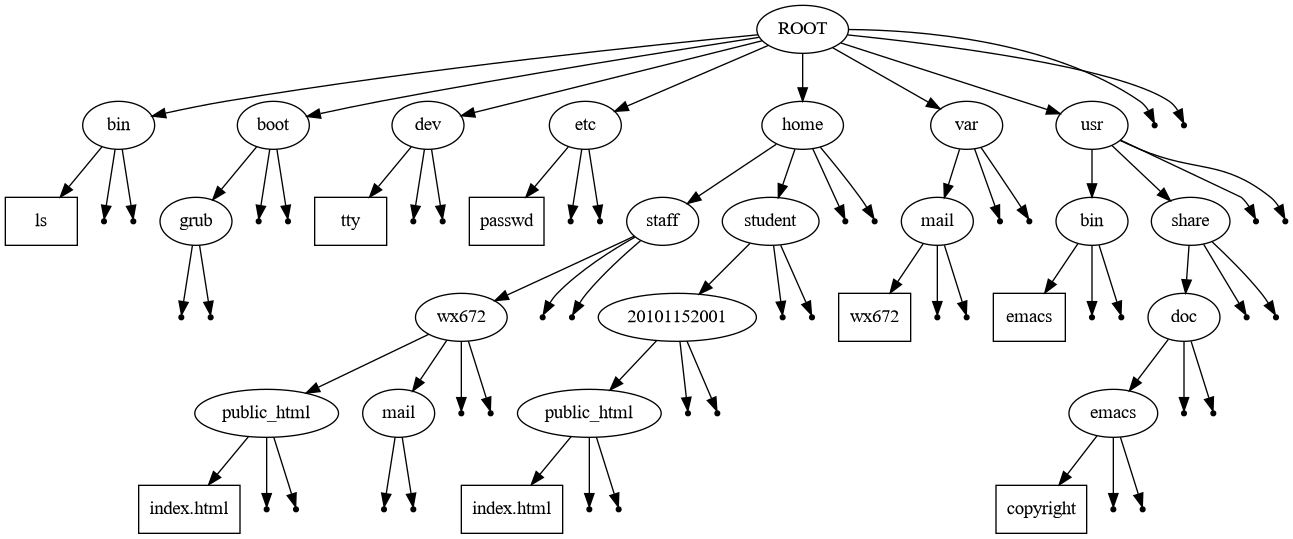
\includegraphics[width=.6\linewidth]{./cs2.png}

\subsection{Must Known Commands}
\label{sec-1-2}
\begin{itemize}
\item \textbf{Simple:}
\begin{verbatim}
ls, cd, pwd, mkdir
cp, mv, rm, ln, chmod
cat, echo, less, more
man, info, help
type, which, whereis
wc, sort, uniq
ps, w, top, free
du, df
ssh, scp
date, cal
\end{verbatim}
\item \textbf{Advanced:}
\begin{verbatim}
grep, find
tar, gzip, 7z 
diff, patch
\end{verbatim}
\end{itemize}
\subsection{CLI shortcuts}
\label{sec-1-3}
\begin{itemize}
\item \textbf{Ctrl-a}: beginning of line
\item \textbf{Ctrl-e}: end of line
\item \textbf{Ctrl-f}: forward
\item \textbf{Ctrl-b}: backward
\item \textbf{Ctrl-n}: next
\item \textbf{Ctrl-p}: previous
\item \textbf{Ctrl-r}: reverse search
\item \textbf{Ctrl-u}: cut to beginning
\item \textbf{Ctrl-k}: kill (cut to end)
\item \textbf{Ctrl-y}: yank (paste)
\item \textbf{Ctrl-d}: delete a character
\end{itemize}
\subsection{Examples}
\label{sec-1-4}
\begin{itemize}
\item \texttt{>} --- output to a file
\begin{verbatim}
date  >  file1
\end{verbatim}
Check what's in \texttt{file1}:
\begin{verbatim}
cat  file1
\end{verbatim}
\item \texttt{>>} --- output a string
\begin{verbatim}
echo Hello, world
\end{verbatim}
output to \texttt{file2} rather than \texttt{STDOUT} (screen)
\begin{verbatim}
echo 'Hello, world!' >> file2
cat file2
echo 'Hello again, world!' > file2
cat file2
\end{verbatim}
\textbf{Q:} Can you explain the difference between \texttt{>} and \texttt{>>}?
\item \texttt{cat} --- concatenate files
\begin{verbatim}
cat file1
cat file2
cat  file1 file2
cat file1 >> file2
cat file2
cat file1 > file2
cat file2
cat >> file2
cat file2
cat > file2
cat file2
\end{verbatim}
\textbf{Q:} Can you explain the above commands?
\item \texttt{ln} --- one file can have several names (shortcuts)
\begin{verbatim}
ln -s file1 file11
ls -l file*
\end{verbatim}
\item \texttt{head} --- list the head (first 10 lines) of file1?
\begin{verbatim}
head file1
\end{verbatim}
\item \texttt{tail} --- list the tail (last 10 lines) of file1?
\begin{verbatim}
tail file1
\end{verbatim}
\item \texttt{cp} --- copy
\begin{verbatim}
cp  file1  file111
ls  -l file*
cp file* /tmp
ls -l /tmp
\end{verbatim}
When copying directories, you need the '\texttt{-a}' option:
\begin{verbatim}
mkdir testdir
cp -a testdir /tmp
\end{verbatim}
\item \texttt{mv} --- move/rename
\begin{verbatim}
mv  file1  file1111
ls  -l  file*
mv file* /tmp
ls -l /tmp/file*
\end{verbatim}
\textbf{Q:} Any differences between \textbf{move} and \textbf{rename}?
\item \textbf{file types}, \textbf{file modes}, and \textbf{file permissions}

Given the following \texttt{ls -l} output:
\begin{verbatim}
lrwxrwxrwx 1  root root 23    May 17  2010 /usr/bin/emacs -> /etc/alternatives/emacs*
-r--r--r-- 1  root sys  418   Oct 13 16:25 /etc/passwd
drwxrwxrwx 10  bin bin  1024  Oct 15 20:27 /usr/local/ 
-r-sr-xr-x 1  root bin  28672 Nov  6  1997 /usr/sbin/ping 
\end{verbatim}
Tell me:
\begin{enumerate}
\item the file type of the above files?
\item the owner and group of the above files?
\item the permissions for the owner, group, and all "other" users of the above files?
\end{enumerate}
\item \texttt{chmod} --- change \textbf{file mode}
\begin{verbatim}
chmod  777  file1  &&  ls  -l  file1
chmod  000  file1  &&  ls -l file1
chmod  a+rwx  file1  &&  ls  -l  file1
chmod  a-rwx  file1  &&  ls  -l  file1
chmod  755  file1  &&  ls  -l  file1
chmod  700  file1  &&  ls  -l  file1
chmod  777  file1  &&  ls  -l  file1
chmod  go-rwx  file1  &&  ls  -l  file1
chmod  600  file1  &&  ls  -l  file1
chmod  u+x  file1  &&  ls  -l  file1      
\end{verbatim}
\item \texttt{wc} --- word count
\begin{verbatim}
wc  -l  file1
\end{verbatim}
\end{itemize}
\section{Shell Basics}
\label{sec-2}
\subsection{Shabang}
\label{sec-2-1}
\begin{verbatim}
#!/bin/sh
#!/bin/bash
#!/usr/bin/python
#!/usr/bin/php
\end{verbatim}
\subsection{Shell variables}
\label{sec-2-2}
\begin{verbatim}
echo  $PATH
echo  $PWD
echo  $HOME
echo  $USER
\end{verbatim}
Try command \texttt{env}, \texttt{set}, \texttt{unset}
\subsection{PATH}
\label{sec-2-3}
\begin{verbatim}
PATH="./:$PATH"
echo $PATH
\end{verbatim}

\subsection{Background and foreground jobs}
\label{sec-2-4}
\begin{itemize}
\item To run a command in the background
\begin{verbatim}
emacs &
google-chrome &
\end{verbatim}
Show background jobs:
\begin{verbatim}
jobs
\end{verbatim}
\item To push a foreground process into background?
\begin{verbatim}
Ctrl-Z
bg %1
\end{verbatim}
\end{itemize}
\subsection{Processes}
\label{sec-2-5}
\begin{verbatim}
ps ux
ps aux
top
w
\end{verbatim}
\subsection{File types}
\label{sec-2-6}
\begin{enumerate}
\item normal files
\item directories
\item links
\item block devices
\item character devices
\item pipes
\item sockets
\end{enumerate}

\textbf{Hint:} the last four can be found in the \texttt{/dev} directory
\subsection{Special files}
\label{sec-2-7}
\begin{itemize}
\item \texttt{/dev/null}
\begin{verbatim}
ls  >  /dev/null
cat  log* nullfile  2>  /dev/null
cat  log* nullfile  &>  /dev/null  
\end{verbatim}
\end{itemize}
\begin{itemize}
\item \texttt{/dev/zero}
\begin{verbatim}
dd  if=/dev/zero  of=/tmp/testfile  bs=1k  count=1000
\end{verbatim}
\item \texttt{/dev/random}
\begin{verbatim}
echo $(( `od -An -N2 -i /dev/random` % 1000 ))
\end{verbatim}
\end{itemize}
\subsection{Soft links and hard links}
\label{sec-2-8}
\begin{verbatim}
ln -s /tmp/a /tmp/aa
ls -l /tmp/a*
ln /tmp/a /tmp/aaa
ln /tmp/aa /tmp/aaaa
ls -li /tmp/a*
\end{verbatim}
\subsection{Getting help}
\label{sec-2-9}
\begin{verbatim}
man -k music player
apropos music player
info tar
\end{verbatim}
\subsection{Advanced commands and concepts}
\label{sec-2-10}
\subsubsection{Pipe --- chaining commands together}
\label{sec-2-10-1}
\begin{verbatim}
man ls | head
man ls | head | tail -3
cat file1 | head -20 | tee file5
\end{verbatim}

\subsubsection{finding a file}
\label{sec-2-10-2}
\begin{verbatim}
find  /  -name  ls
type  ls
which  ls
whereis ls
find  /etc  -type d -name "rc*"
find ~ -name "*~" | xargs rm
\end{verbatim}

\subsubsection{grep --- finding lines in files}
\label{sec-2-10-3}
\begin{verbatim}
grep stud /etc/passwd
man cp | grep -B2 -A2 recur
\end{verbatim}

\subsubsection{Single-quotes and double-quotes}
\label{sec-2-10-4}
\begin{verbatim}
a=alpha;  b="$a";  c='$a'
echo  a  b  c
echo  $a $b $c
echo '$a $b $c'    
echo "$a $b $c"
\end{verbatim}

\subsubsection{Wildcard charactors}
\label{sec-2-10-5}
\begin{verbatim}
mkdir  tmp  &&  cd  tmp
for  ((i=0;i<101;i++));  do  touch  f$i;  done
ls  f*
ls  f?
ls  f??
ls  ??
ls  ?8*
ls  *0
\end{verbatim}

\subsubsection{Command alias}
\label{sec-2-10-6}
\begin{verbatim}
alias
alias la='ls -a'
alias rm='rm -i'
which rm
\end{verbatim}

\subsubsection{\texttt{STDIN}, \texttt{STDOUT}, \texttt{STDERR}, and redirection (\texttt{>}, \texttt{>>}, \texttt{<})}
\label{sec-2-10-7}
\begin{itemize}
\item Redirect \texttt{STDOUT} into a file
\begin{verbatim}
ls  >  listing
cat  listing  >  listing2
cat  listing*  >  listing3
cat  listing* >> listing3
\end{verbatim}
\item Redirect \texttt{STDIN} from a file
\begin{verbatim}
cat  <  listing
sort  <  listing
\end{verbatim}
\begin{minted}[mathescape=true,linenos=true,numbersep=5pt,frame=lines,framesep=2mm]{bash}
#!/bin/bash
while  read  LINE
do
  case  $LINE  in  
  *root*)  echo  $LINE ;;
  *stud*)  echo  $LINE ;;
       *)  echo  "I don't care." ;;
  esac 
done  <  /etc/passwd
\end{minted}
\item Redirect \texttt{STDERR} into a file
\begin{verbatim}
touch  realfile
ls  nullfile  realfile
\end{verbatim}

\begin{verbatim}
ls  nullfile  realfile  2>  log2
ls  2>  log  nullfile  realfile
\end{verbatim}
\item Redirect both \texttt{STDERR} and \texttt{STDOUT} into a file
\begin{verbatim}
ls  nullfile  realfile  &>  log3
ls  nullfile  realfile  > log3  2>&1
\end{verbatim}

\begin{verbatim}
diff  log*
\end{verbatim}

\begin{verbatim}
cat  nullfile  realfile  &>  log4
cat  &>  errorlog  <  nullfile realfile
\end{verbatim}
\end{itemize}

\subsubsection{Initial files}
\label{sec-2-10-8}
\begin{itemize}
\item \texttt{.bashrc}, \texttt{.bash\_profile}, \texttt{.profile}
\begin{verbatim}
vim  .bashrc
source  .bashrc
.  .bashrc
\end{verbatim}
\end{itemize}

\subsubsection{tar}
\label{sec-2-10-9}
\begin{verbatim}
tar  cvf  myarchive.tar  /etc/termcap  /etc/passwd
tar  tvf  myarchive.tar
tar  xvf  myarchive.tar
\end{verbatim}
With compression:
\begin{verbatim}
tar  zcvf  myarchive.tgz  /etc/termcap  /etc/passwd
tar  zxvf  myarchive.tgz
tar  ztvf  myarchive.tgz
\end{verbatim}

\subsubsection{gzip}
\label{sec-2-10-10}
\begin{verbatim}
gzip file1
zcat file1.gz
gunzip file1.gz
\end{verbatim}

\subsubsection{System info}
\label{sec-2-10-11}
\begin{verbatim}
mount
uname -a
dmesg
lspci
lsusb
lsmod
\end{verbatim}

\subsubsection{Job scheduling}
\label{sec-2-10-12}
\begin{itemize}
\item \texttt{at}
\begin{verbatim}
at  11:00
at>  date >> $HOME/date.out
at>  type CTRL-D to quit
at -l
\end{verbatim}
\item \texttt{crontab}
\begin{verbatim}
crontab -e
*/2 * * * * date  >>  $HOME/date.out
crontab -l
\end{verbatim}
\end{itemize}
\section{Bash Programming Examples}
\label{sec-3}
\subsection{\texttt{for} VAR \texttt{in} LIST; \texttt{do} SOMETHING; \texttt{done}}
\label{sec-3-1}
\begin{minted}[mathescape=true,linenos=true,numbersep=5pt,frame=lines,framesep=2mm]{bash}
for i in 1 2 3 4 5; do echo $i; done
for ((i=1;i<6;i++)); do echo $i; done
\end{minted}
\begin{minted}[mathescape=true,linenos=true,numbersep=5pt,frame=lines,framesep=2mm]{bash}
for i in 1 2 3 4 5; do echo $((i*i)); done
for ((i=1;i<6;i++)); do echo $((i*i)); done
\end{minted}
\begin{minted}[mathescape=true,linenos=true,numbersep=5pt,frame=lines,framesep=2mm]{bash}
for i in 1 2 3 4 5; do j=$((i*i)); echo $i $j; done
for ((i=1;i<6;i++)); do j=$((i*i)); echo $i $j; done
\end{minted}
\begin{minted}[mathescape=true,linenos=true,numbersep=5pt,frame=lines,framesep=2mm]{bash}
#!/bin/bash
# check disk usage.
for f in /home/students/*
do
  du -cks $f | grep -v total
done | sort -n | tail -10
\end{minted}
\begin{minted}[mathescape=true,linenos=true,numbersep=5pt,frame=lines,framesep=2mm]{bash}
for f in /home/stud/*; do du -b $f; done | sort -n | tail -10
du -b /home/stud/* | sort -n | tail -10
\end{minted}
\begin{minted}[mathescape=true,linenos=true,numbersep=5pt,frame=lines,framesep=2mm]{bash}
for f in *jpg; do convert $f -resize 1280x -gravity center -crop 1280x768+0+0 `basename $f .jpg`-1280x768.jpg; done
\end{minted}
\subsection{\texttt{if} TEST; \texttt{then} COMMANDS; \texttt{else} OTHERCOMMANDS; \texttt{fi}}
\label{sec-3-2}
\subsubsection{Comparisons}
\label{sec-3-2-1}
\begin{minted}[mathescape=true,linenos=true,numbersep=5pt,frame=lines,framesep=2mm]{bash}
if [ $a -lt 10 ];   then a=$(($a+1)); echo $a; else echo "a is too large."; fi

if [[ $a -lt 10 ]]; then a=$(($a+1)); echo $a; else echo "a is too large."; fi

if (("$a" < 10));   then a=$(($a+1)); echo $a; else echo "a is too large."; fi
\end{minted}
\begin{minted}[mathescape=true,linenos=true,numbersep=5pt,frame=lines,framesep=2mm]{bash}
#!/bin/bash
# This is a simple string comparision script.
#
# 1. Use '[[' instead of '[' whenever possible.
# 2. Don't use '[  ]' with '<', '>'.
# 3. '-eq -le -ge -lt -gt' are for arithmetic comparisons
# 4. '< >' for string comparisons
#
if [ -z "$2" ]; then
    echo Usage: $0 '<string1> <string2>'
elif [[ "$1" > "$2" ]]; then
    echo $1 is bigger than $2.
elif [[ "$1" = "$2" ]]; then
    echo $1 is equal to $2.
else
    echo $1 is smaller than $2.
fi
\end{minted}
\begin{minted}[mathescape=true,linenos=true,numbersep=5pt,frame=lines,framesep=2mm]{bash}
if [[ $(ls | wc -l) -gt 10 ]]; then echo "messy!"; else echo "clean!"; fi
\end{minted}
\begin{itemize}
\item \href{http://www.tldp.org/LDP/abs/html/comparison-ops.html}{Other Comparison Operators}
\end{itemize}
\subsubsection{Test exit status}
\label{sec-3-2-2}
\begin{minted}[mathescape=true,linenos=true,numbersep=5pt,frame=lines,framesep=2mm]{bash}
#!/bin/bash
for f in *.sh
do
    if grep -q while $f; then
	echo "$f: while loop found\!"
    else
	echo "$f: no while loop."
    fi
done
\end{minted}
\begin{minted}[mathescape=true,linenos=true,numbersep=5pt,frame=lines,framesep=2mm]{bash}
if grep -q while while.sh ; then echo "While loop found."; else echo "no while loop"; fi
\end{minted}
\begin{minted}[mathescape=true,linenos=true,numbersep=5pt,frame=lines,framesep=2mm]{bash}
for f in *.sh; do if grep -q while $f; then echo "$f: while loop found\!"; else echo "$f: no while loop"; fi; done
\end{minted}
\subsubsection{See your \texttt{.bash\_profile}}
\label{sec-3-2-3}
\begin{minted}[mathescape=true,linenos=true,numbersep=5pt,frame=lines,framesep=2mm]{bash}
# include .bashrc if it exists
if [ -f ~/.bashrc ]; then
   . ~/.bashrc
fi
# set PATH so it includes user's private bin if it exists
if [ -d ~/bin ] ; then
   PATH=~/bin:"${PATH}"
fi
\end{minted}
\subsection{\texttt{while} CONDITION; \texttt{do} SOMETHING; \texttt{done}}
\label{sec-3-3}
\begin{minted}[mathescape=true,linenos=true,numbersep=5pt,frame=lines,framesep=2mm]{bash}
while true; do mpg123 song.mp3; done

while true; do mpg123 `find ~/ -iname "*.mp3"`; done
\end{minted}
\begin{minted}[mathescape=true,linenos=true,numbersep=5pt,frame=lines,framesep=2mm]{bash}
#!/bin/bash
x=0 
while [ $x -lt 10 ]      #  [ ]
do 
    y=$x 
    while [[ $y -ge 0 ]]   #  [[ ]]
    do 
	echo -n $y         # no newline
	y=$((y-1))         # y--
    done 
    echo 
    x=`echo "$x + 1" | bc` # x++
done
\end{minted}

\subsubsection{\texttt{read} --- Read a line from STDIN}
\label{sec-3-3-1}
\begin{minted}[mathescape=true,linenos=true,numbersep=5pt,frame=lines,framesep=2mm]{bash}
while read LINE; do echo "what I typed is: $LINE"; done
\end{minted}
\begin{minted}[mathescape=true,linenos=true,numbersep=5pt,frame=lines,framesep=2mm]{bash}
#!/bin/bash
while read LINE
do
    case $LINE in  
	*root*) echo $LINE ;;
	*stud*) echo $LINE ;;
	*) echo "I don't care." ;;
    esac 
done < /etc/passwd
\end{minted}
\subsection{\texttt{case} VAR \texttt{in} PATTERN) COMMANDS ;; \texttt{esac}}
\label{sec-3-4}
\begin{minted}[mathescape=true,linenos=true,numbersep=5pt,frame=lines,framesep=2mm]{bash}
#!/bin/bash
printf "Play a game?" 
read YN 
case $YN in 
  [yY]|[yY][eE][sS]) exec bb ;; 
		  *) echo "Maybe later." ;; 
esac
\end{minted}
\begin{minted}[mathescape=true,linenos=true,numbersep=5pt,frame=lines,framesep=2mm]{bash}
#!/bin/bash
YN=yes 
printf "Play a game?[$YN]" 
read YN 
: ${YN:=yes}
case $YN in 
  [yY]|[yY][eE][sS]) exec bb ;; 
		  *) echo "Maybe later." ;; 
esac
\end{minted}
\subsection{Command line arguments (\texttt{\$0, \$1, \$2...}, \texttt{\$\#, \$@})}
\label{sec-3-5}

\begin{listing}[H]
\begin{minted}[mathescape=true,linenos=true,numbersep=5pt,frame=lines,framesep=2mm]{c}
#include <stdio.h>

int main(int argc, char *argv[])
{
  int i;
  printf("You said:\n\t");

  for(i=1; i<argc; i++)
    printf("%s ",argv[i]);

  printf("\n\n\targc = %d\n", argc);

  for(i=0; i<argc; i++)
    printf("\targv[%d] = %s\n",i,argv[i]);

  return 0;
}
\end{minted}
\caption{An example C program:}
\end{listing}

\begin{listing}[H]
\begin{minted}[mathescape=true,linenos=true,numbersep=5pt,frame=lines,framesep=2mm]{bash}
#!/bin/bash

echo "You said:"

echo -e "\t$@"
echo
echo -e "\targc = $#"
echo -e "\targv[0] = $0"

i=1
for arg in $@; do
    # printf "arg[$i] is %s\n" "$arg"
    echo -e "\targv[$i] = $arg"
    let i++
done
\end{minted}
\caption{An equivalent bash script:}
\end{listing}

\subsection{Arrays}
\label{sec-3-6}
Set random wallpaper:
\begin{minted}[mathescape=true,linenos=true,numbersep=5pt,frame=lines,framesep=2mm]{bash}
#!/bin/bash
### demonstrate ARRAY and RANDOM ###

files=($HOME/pics/2009summer/wallpapers/2009summer-1280x768/*.jpg)

# get the length of array ${files[@]}
n=${#files[@]}

# get a random array element
wallpaper="${files[RANDOM % n]}"

# set it as wallpaper
qiv -z $wallpaper
\end{minted}

\subsection{GUI}
\label{sec-3-7}
\begin{minted}[mathescape=true,linenos=true,numbersep=5pt,frame=lines,framesep=2mm]{bash}
#!/bin/bash
while NAME=`zenity --entry --text="Your name?"` 
do
    zenity --info --text="Hello, $NAME\!"
done
\end{minted}

\subsection{\texttt{/etc/init.d/*}}
\label{sec-3-8}
Check files in \texttt{/etc/init.d/} directory to see how shell scripts can be used seriously.
Emacs 24.5.1 (Org mode 8.2.10)
\end{document}